\documentclass[Main]{subfiles}

\begin{document}

\chapter{Scope}

\section{Identification}
This Request for Proposal (RFP) identifies, specifies and establishes the detailed system requirement for the Self-Protection Suite POD structure (SPS-POD).

\section{System overview}
The purpose of the SPS is to provide Royal Danish Air Force with a self-protection suite for the F-16 combat aircraft. 
The system will provide warning upon detection of missile threats and automatically dispense payloads in response.

\begin{figure}[hbtp]
\centering
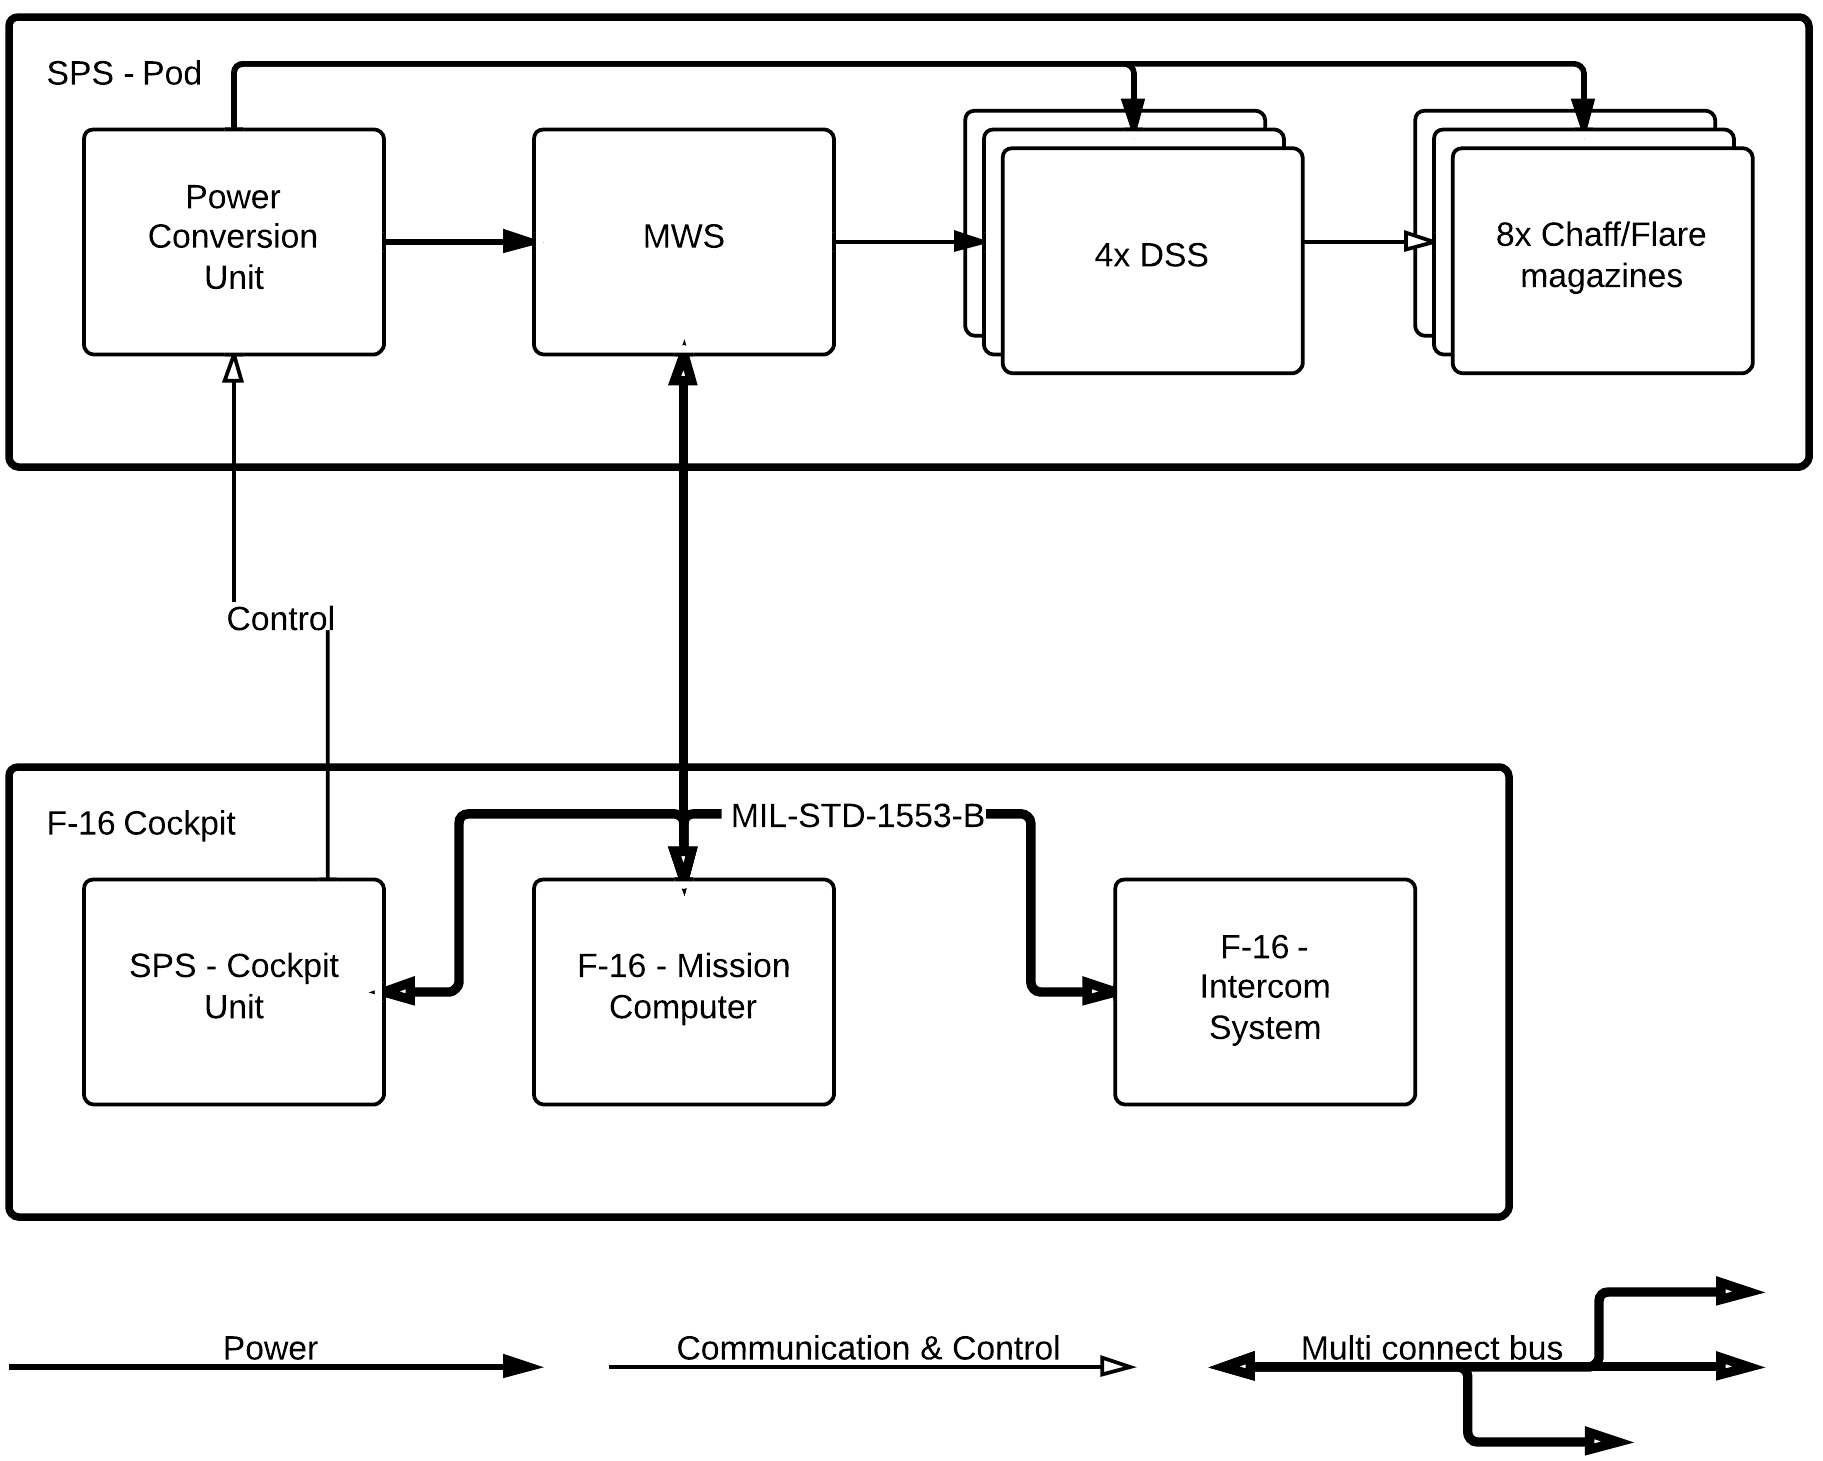
\includegraphics[width = 0.9\textwidth]{ConceptOfOperations}
\caption{Concept of Operations of Self Protection Suite}
\label{fig:conOps}
\end{figure}

The SPS-POD (see Figure ~\ref{fig:conOps}) will host a Missile Warning System, Chaff/flare magazines, digital sequencer switches and a Power Conversion Unit. 
It will be mounted on the left hand wing of th F-16 combat aircraft.

\section{Scope of Delivery}
The system to be delivered is the pod structure itself with facilities and wiring for installing required subsystems. 
Production of all control systems and integration of MWS, PCU, DDS's and magazines will be done by Terma.

If the pod structure itself cannot comply with given thermal requirements (see Section ~\ref{sec:SER}), a climate control system must be constructed, supplied and integrated by the sub-supplier.

\section{Document overview}
This section has been tailored out. See Table of Contents.

\subfile{Abbreviations}

\end{document}
